\documentclass[a4paper, 11pt]{tubsreprt}
\usepackage[ngerman]{babel}
\usepackage[utf8]{inputenc}
\usepackage{cite}
\usepackage{graphicx}
\usepackage{wrapfig}
\title{Wärmebehandlung}
\date{Wintersemester 17/18}
\author{J. Hansen, S. Vodde,
 J. Veer, T. Stein}

\logo{
	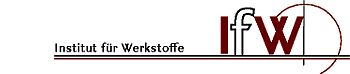
\includegraphics{Bilder/ifw-logo.jpg}
}

\begin{document}
\maketitle
\tableofcontents
\chapter{Titanwerkstoffe}

\section{Gefügemerkmale}
Wie andere Metalle liegt Titan in verschiedenen Gittermodifikationen beziehungsweise Phasenzuständen vor. Der Zustand ist von der Temperatur und den vorliegenden Legierungselementen abhängig. Bei reinem Titan liegt zwischen 1668°C und 882°C ein kubisch raumzentriertes Kristallgitter vor. Diese Phase wird als Betaphase ($\beta$-Phase) bezeichnet. Bei 882°C erfährt Titan eine Phasenumwandlung zu einem hexagonalen Gitter. Diese Phasenumwandlungstemperatur wird als Betatransus Temperatur bezeichnet und ist für jede Legierung unterschiedlich, denn die Legierungselemente haben Einfluss auf diese. \cite{Luetjering2007}.

Das hexagonale Gitter wird als Alphaphase ($\alpha$-Phase) bezeichnet. Wenn das Material langsam abgekühlt ist, liegt reines Titan bei Raumtemperatur nahezu vollständig als Alphaphase vor. 

Dieses Gitter der Alphaphase ist annähernd dichtest gepackt. Das Verhältnis in der Zelle ist etwas kleiner, als dass in der am dichtesten gepackten Zelle, c:a von $\alpha$-Titan liegt bei 1.586. Die perfekte hexagonale Zelle hat ein Verhältnis von 1.624 \cite{Siemers2017}, wobei c und a die Längen innerhalb einer Zelle sind. Je nach Aufbau der Zelle sind diese Längen unterschiedlich groß.

Die Phasenumwandlung zwischen $\beta$- und $\alpha$-Phase kann auch martensitisch erfolgen. Dabei muss das Material aus einer ausreichend hohen Temperatur abgeschreckt werden. Diese Temperatur wird als Martensitstarttemperatur bezeichnet. Sie ist wie die Betatransustemperatur von den Legierungselementen abhängig.  

\subsection{Alpha-Titan Phase}
Die alpha-Titan Phase ist durch eine hexagonale Gitterstruktur gekennzeichnet. Dadurch entsteht ein anisotropes Werkstoffverhalten in einem Korn, beziehungsweise Einkristall.
Ein Einkristall ist über ein homogenes, einheitliches Kristallgitter definiert.
In einem Belastungsfall dieses Einkristalls ist das Werkstoffverhalten abhängig von der Belastungsrichtung im Verhältnis zur Gitterrichtung. Eine Kenngröße, die das elastische Verhalten eines Werkstoffes definiert, ist das Elastizitätsmodul: 
\begin{equation}
E=\sigma*\epsilon
\end{equation}
Das Elastizitätsmodul ist das Verhältnis zwischen der anliegenden Spannung $\sigma$ und die dadurch resultierende Dehnung $\epsilon$.
Es wird in Pascal angegeben. Das Elastizitätsmodul $E$ reicht je nach Verhältnis, von minimal 100 GPa bis maximal 145 GPa. 

Jedoch wird Titan sehr selten als Einkristall hergestellt, sodass die unterschiedliche Kornorientierung dafür sorgt, dass die anisotropie der einzelnen Körner sich gegenseitig aufhebt. Somit kann man von einem isotropen Werkstoffverhalten ausgehen.

\subsection{Beta-Titan Phase}
Eine $\beta$-Phase ist ein Gefüge mit einer kubisch raumzentrierten Gitteranordnung. Dadurch resultiert ein homogenes Werkstoffverhalten.

Eine große Menge an $\beta$-Phase existiert in der Regel bei Raumtemperatur nur unter bestimmten Bedingungen. Sie kann als metastabile Phase auftreten, was bedeutet, dass das Material nicht vollständig den Phasenübergang abschließen konnte und so in dem Zustand aus höheren Temperaturen verblieben ist.  

Durch Zusatz bestimmter Legierungselemente kann die $\beta$-Phase auch in größeren Mengen vorliegen. Dies wird im Kapitel betastabilisierende Legierungselemente näher erläutert.
\subsection{Gefüge}
Ausgehend von grundlegend verschiedenen Gefügen können diese durch Wärmebehandlung hinsichtlich ihrer mechanischen Eingenschaften optimiert werden. Eine Kombination aus mehreren Gefügeausprägungen können die Vorteile der einzelnen kombinieren. Dazu werden mehrstufige Wärmebehandlungen eingesetzt. Die mögliche Wärmebehandlung, zum einstellen der Gefüge, findet nach der Rekristallisation statt, sodass einige Gefügeausbildungen eventuell nicht möglich sind. Dies hängt von dem Ausgangsgefüge ab.
\subsubsection{Lamellar}
Lamellare Gefüge sind unabhängig von dem Ausgangsgefüge einstellbar.Sie entstehen aus einer Abkühlung aus dem $\beta$-Gebiet. Während des Abkühlens bilden sich in den Korngrenzen der $\beta$-Phase $\alpha$-Bereiche, die in das $\beta$-Korn hinein wachsen. Die Alphabereiche wachsen erst in eine Richtung bevor sie ihre Dicke erhöhen. Je nach Abkühlgeschwindigkeit entstehen so dünne oder dickere Nadeln. Die Abbildung 1.1 zeigt ein beispielhaftes Gefüge, indem voll lamellare Strukturen zu sehen sind und wird auch als Widmannstättengefüge bezeichnet. 


\begin{figure}


	\centering
		\includegraphics[scale=1]{Bilder/lamellar.jpg}
		\captionof{figure}[lamellares Gefüge]{Volllamellares Gefüge \cite{Leyens2002}}
		\label{fig1}
		
\end{figure}
\subsubsection{Martensit}
Der Martensit ist eine spezielle Form unter den Gefügen, da dieser der einzige ist in denen die Phasen metastabil vorliegen. Er resultiert aus einer schnellen Abkühlung bei Temperaturen höher als als die Martensitstarttemperatur. Bei diesen Temperaturen ist das Volumenverhältnis zwischen $\alpha$ und $\beta$ in dem diese stabil vorliegen ein anderes als das bei niedrigen Temperaturen. Bei einer langsamen Abkühlung würde sich die Betaphase in Alphaphase umwandeln. Aufgrund der schnellen Abkühlgeschwindigkeit von über 1000°C/min können diese Diffusionsvorgänge nicht abgeschlossen werden. Somit kommt es zu einem diffuisonslosen Phaseübergang. Aufgrund der unterschiedlichen Gitterstruktur von Alpha und Beta, kommt es zu dem charakteristischen Martensitgefüge wie in Abbildung 1.2 zu sehen ist.

\begin{figure}
\centering
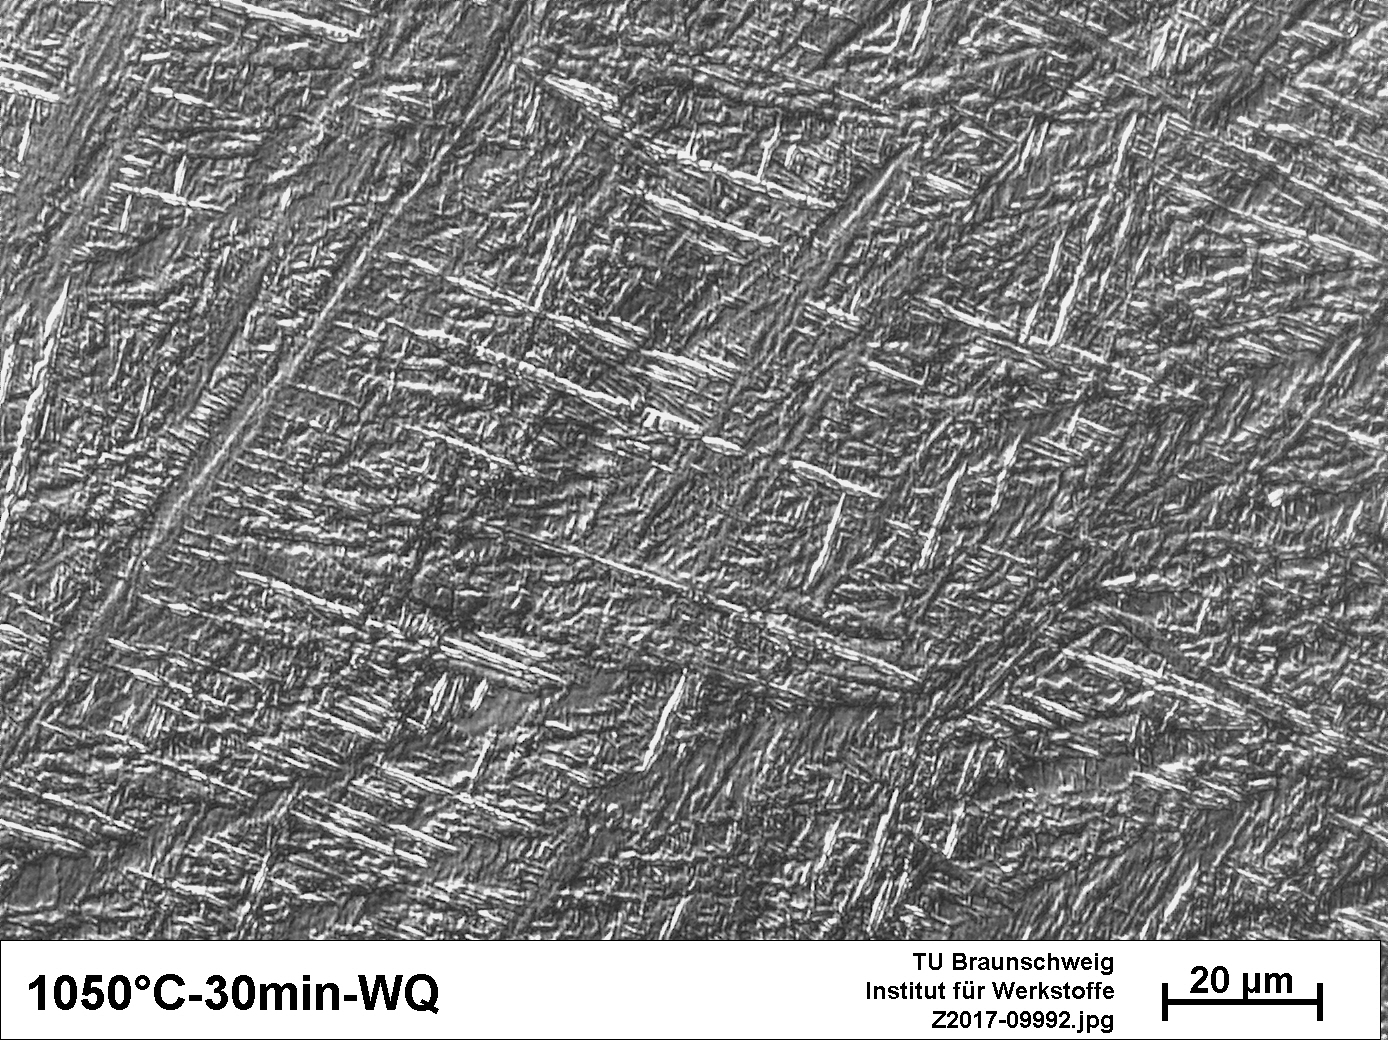
\includegraphics[scale=0.5]{Bilder/Vollmartensit.jpg}
\caption{Vollmartensitisches Gefüge}
\label{fig3}
\end{figure}
\subsubsection{Globular}


\subsubsection{Bi-Modal}
Bi-Modal-Gefüge(Duplex-Gefüge) sind durch globularer $\alpha$-Phase und Lamellen aus $\alpha$- und $\beta$-Phase gekennzeichnet. Das Gefüge kombiniert rein globulare Alphaphase mit lamellaren Anteilen. In Abbildung 1.3 ist ein solches Gefüge zu erkennen. Viele 
\begin{figure}
\centering
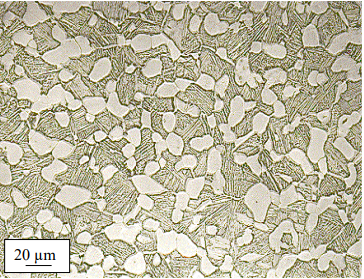
\includegraphics[scale=1]{Bilder/Duplexgefuege.PNG}
\caption[Bi-Modal-Gefüge]{Bi-Modal-Gefüge\cite{Werkstoffdesign2012}}
\label{fig4}
\end{figure}

\chapter{Methodik}
\section{Wärmebehandlung}

Die Wärmebehandlung nach der Rekristllisation ist die letzte Methode um das Gefüge des Titans einzustellen. Hierbei kommt es auf Parameter wie Temperatur, Haltezeit und Abkühlmethode an. Um die bereits erwähnten Gefüge zu realisieren, ist eine spezifische Abfolge von einer beziehungsweise mehreren Stufen einer Wärmebehandlung nötig. Die grundlegenden Behandlungen werden in diesem Kapitel behandelt, wobei die speziellen, mehrstufigen Behandlungen im dritten Kapitel behandelt werden.
\paragraph{Temperaturkontrolle}
Für die Temperaturkontrolle innerhalb der Wärmebehandlung kam ein Ofen zum Einsatz. Dieser kann bis Temperaturen weit über Betatransus (genaue Zahl) aufheizen und diese, mit einer Genauigkeit von drei Kelvin, halten. Der Ofen ist außerdem für die Aufheizgeschwindigkeit verantwortlich, da diese auch einen wichtigen Einfluss haben kann.
\paragraph{Abkühlmedien}

Durch Abkühlmedien werden bestimmte Abkühlgeschwindigkeiten realisiert. Für langsamere Abkühlungen als in der Luft wird der Ofen genutzt. Hier kann die Temperatur beliebig langsam reduziert werden. Ein weiterer Vorteil des Ofens ist, dass die Probe auf eine bestimmte Temperatur herunter gekühlt werden kann. Dies ist für mehrstufige Wärmebehandlungen wichtig, bei denen eine Abkühlung auf Raumtemperatur zwischen den Schritten vermieden werden soll. 

Da der Ofen nicht überaus schnell abkühlen kann, wird zur schnelleren Abkühlung Luft mit Raumtempertur verwendet. Durch den höheren Temperaturgradienten im Verhältnis zum Ofen wird so die Abkühlung beschleunigt.  

Um noch schnellere Abkühlungen zu realisieren wird Wasser oder Öl verwendet. So werden zum Beispiel Abkühlgeschwindigkeiten für eine Martensitbildung ermöglicht. Die hohe Abkühlgeschwindkeit von gewöhnlich mehr als 1000°C/min verhindert das elemente partitioning. So können sich neben dem Martensit, Alpha-Beta-Verhältnisse einstellen, die bei langsamen Abkühlungen nicht möglich sind. 
\subsection*{Anpassung der Gefüge durch Wärmebehandlung}
\begin{figure}
	\centering
	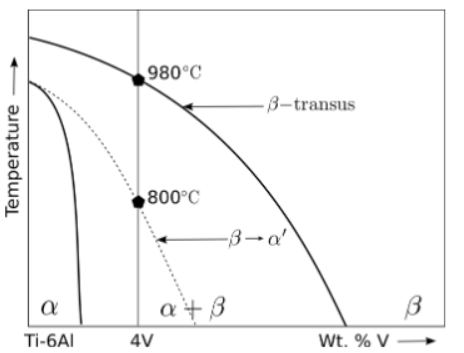
\includegraphics[scale=0.9]{Bilder/Phasendiagram.PNG}
	\caption[Phasendiagramm]{schematisches Phasendiagramm Ti-6Al-4V \cite{Babu2008}}
	\label{fig2}
\end{figure}
Das Anpassen der Gefüge ist das Ziel der Wärmebehandlungen. So werden Werkstoffeigenschaften gezielt für den jeweiligen Anwendungsfall optimiert, denn bestimmte Gefüge folgen aus bestimmten Wärmebehandlungen. 

\bibliographystyle{plain}
\bibliography{literatur}
\listoffigures
\listoftables
\end{document}
